% Copyright 2014 Joakim Nilsson
%
% This text is free software: you can redistribute it and/or modify
% it under the terms of the GNU General Public License as published by
% the Free Software Foundation, either version 3 of the License, or
% (at your option) any later version.
%
% This text is distributed in the hope that it will be useful,
% but WITHOUT ANY WARRANTY; without even the implied warranty of
% MERCHANTABILITY or FITNESS FOR A PARTICULAR PURPOSE.  See the
% GNU General Public License for more details.
%
% You should have received a copy of the GNU General Public License
% along with this text.  If not, see <http://www.gnu.org/licenses/>.

% Document class
\documentclass[a4paper]{article}

% Packages
\usepackage{hyperref}
\usepackage[utf8]{inputenc}
\usepackage{graphicx} % For \rotatebox
\usepackage{tabularx}
\usepackage{pbox}

% Commands
\newcommand{\rotccw}[1] {
	\rotatebox{90}{{#1}}
}

% Title
\title{Combo Whist}
\author{By Joakim Nilsson}
\date{Version 1.0 - \today}

% Document
\begin{document}
	% Title
	\maketitle
	
	\begin{center}
		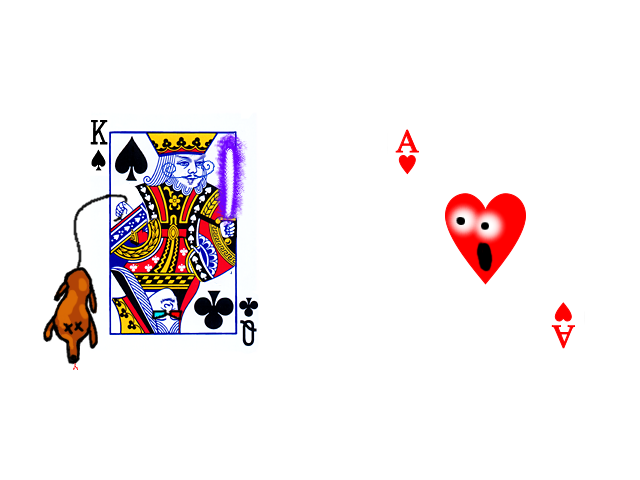
\includegraphics[width = \textwidth]{logo.png}
	\end{center}
	
	\thispagestyle{empty}
	\pagebreak
	
	% Table of contents
	\setcounter{tocdepth}{3}
	\tableofcontents
	\thispagestyle{empty}
	\pagebreak
	
	\section{Overview}
		\subsection{Type of game}
		Card game, Whist
		
		\subsection{Number of players}
		4 is preferred. 3 is possible. More is possible with additional rules.
		
		\subsection{Requirements}
		\begin{itemize}
			\item a standard 52 card deck
			\item pen and paper
		\end{itemize}
		
		\subsection{Difficulty level}
		Somewhere between high and medium. Still not very difficult to learn, however, hard to master.

	\section{The game}
		\subsection{Preparation}
		First, one of the players is chosen by vote to be the dealer. If no majority is formed, the dealer is selected at random. On the paper, one column per player is drawn. Here each players' score and some additional information to be explained later are to be written down.

		\subsection{The deal}
		There are 2 main parts of a deal. The first is the bidding process and the second is the play. The play is described before the bidding process as some information about the play is required to understand the bidding process. However, the deal starts by the dealer, who deals 13 cards to each player (or 17, if there are only 3 players, whereas also the 2 of clubs is removed from the deck before the game starts). After the play, one notes all players scores and a new deal starts with a new dealer (the player to the left of the previous dealer).
			\subsubsection{The play}
			The play is very similar to the common play in a Whist card game. The player to the right of the declarer (The term \emph{declarer} is explained in the ``The bidding process'' section.) begins by playing a card. Then the player to the left of him plays another card which must follow the suite of the first card. Then the next player (the player to the left of the second player) plays yet another card which must also follow the first card's suite, and so on until all players have played one card each. If a player doesn't have a card in the leading suite, he may discard any card or play a trump. There is no obligation to play a trump. The player who played the highest card in the leading suite takes the book (that is, takes all the played cards and puts them face down on the table by himself) unless a trump is played. In the latter case, the player who played the highest trump takes the book. Thereafter, the player who took the book plays the first card and the play goes on until all cards has been played.
			
			\subsubsection{The bidding process}
			In Combo Whist players make combo bids. A combo bid is a bid composed of one standard bid and any amount of different extra bids. The different bids have different rules to be obeyed during the play assigned to them. The players takes turns by bidding in a clockwise pattern and the player to the left of the dealer begins. One can either make a combo bid (from here on simply referred to as a \emph{bid}) which has a higher value than the previous bid or pass. If a player passes, he's out of the bidding process and may therefore not make any new bids until the next deal. A bid's value is the sum of the standard bid's and the extra bids' values and must always be greater than 0. A proposed time limit between each bid is 1 minute, but for beginners a higher limit or no limit is recommended. The bidding process continues until all players but one have passed. That player becomes \emph{declarer} and the play starts. The available standard bids and extra bids are listed in tables \ref{tab:standardBids} and \ref{tab:extraBids}, respectively. The number of books to bring home is specified in the standard bids table in the ``Books'' column and in some cases under the ``Specific rules'' column. An extra bid cannot be bid in combination with another bid listed in the ``Incompatibility'' column. Note that there is a difference between \emph{value} and \emph{score}, where \emph{value} is the bid's value (You guessed it!) and \emph{score} is the number of points the declarer scores if he completes the bid. The standard bids marked with an asterisk (*) have modified rules assigned to them when there are only 3 players participating in the game. These bids are listed in table \ref{tab:standardBids3}.
			
			% Bid tables
			% This file is part of Combo Whist.
%
% Copyright 2007-2016 Joakim Nilsson
%
% This text is free software: you can redistribute it and/or modify
% it under the terms of the GNU General Public License as published by
% the Free Software Foundation, either version 3 of the License, or
% (at your option) any later version.
%
% This text is distributed in the hope that it will be useful,
% but WITHOUT ANY WARRANTY; without even the implied warranty of
% MERCHANTABILITY or FITNESS FOR A PARTICULAR PURPOSE.  See the
% GNU General Public License for more details.
%
% You should have received a copy of the GNU General Public License
% along with this text.  If not, see <http://www.gnu.org/licenses/>.

\begin{table}
	\caption{Standardbud}\label{tab:standardBids}
	\begin{center}
		\begin{tabularx}{\textwidth}{lcccc|X}
				\textbf{Namn} &
				\rotccw{\textbf{Värde}} &
				\rotccw{\textbf{Poäng}} &
				\rotccw{\textbf{Trumf}} &
				\rotccw{\textbf{Stick}} &
				\textbf{Tilläggsregler}
				\\[-3ex]

				\standardBidItem%
				{Dumskipp}
				{$0$}
				{$1$}
				{nej}
				{varierar}
				{%
					Spelföraren får inte ta hem flest stick --- inte ens om nån annan spelare har tagit hem lika många stick.
				}

				\standardBidItem%
				{Ungefär}
				{$1$}
				{$1$}
				{nej}
				{varierar}
				{%
					Före spelets början gissar spelföraren på två möjliga mängder stick denne kommer att ta hem. Hen måste ta hem en av de två möjliga mängderna som gissades.
				}

				\standardBidItem%
				{Trumf*}
				{$1$}
				{$1$}
				{ja}
				{min 5}
				{%
					Spelföraren bestämmer trumffärg.
				}

				\standardBidItem%
				{Grill*}
				{$1$}
				{$2$}
				{ja}
				{min 5}
				{%
					Spelföraren börjar med att bestämma trumffärg. Denna trumffärg gäller bara första sticket. Därefter blir den färg som spelades ut i föregångde stick ny trumffärg och så fortsätter det till spelets slut.
				}
				
				\standardBidItem%
				{Spader*}
				{$2$}
				{$1$}
				{ja}
				{min 5}
				{%
					Trumffärgen är spader.
				}

				\standardBidItem%
				{Spel*}
				{$2$}
				{$2$}
				{nej}
				{min 5}
				{%
					---
				}

				\standardBidItem%
				{Skipp*}
				{$3$}
				{$2$}
				{nej}
				{varierar}
				{%
					Spelföraren måste ta hem färst stick. Om ingen tar hem färre stick än spelföraren går budet hem.
				}

				\standardBidItem%
				{Exakt}
				{$3$}
				{$2$}
				{nej}
				{varierar}
				{%
					Före spelets början gissar spelföraren på en möjlig mängd stick denne kommer att ta hem. Hen måste ta hem den mängd som gissades.
				}

				\standardBidItem%
				{Maxtrumf*}
				{$3$}
				{$3$}
				{ja}
				{min 7}
				{%
					Spelföraren väljer trumffärg.
				}

				\standardBidItem%
				{Smygtrumf*}
				{$3$}
				{$3$}
				{ja}
				{min 5}
				{%
					Spelföraren väljer trumffärg. Hen får dock inte välja en trumffärg som hen har flest kort i.
				}

				\standardBidItem%
				{Mästarspel}
				{$4$}
				{$3$}
				{nej}
				{varierar}
				{%
					Spelföraren måste ta hem flest stick. Om denna tar hem lika många som nån annan spelare så går budet inte hem.
				}

				\standardBidItem%
				{Noll}
				{$4$}
				{$4$}
				{nej}
				{0}
				{%
					---
				}

				\standardBidItem%
				{Mästartrumf*}
				{$6$}
				{$6$}
				{ja}
				{min 5}
				{%
					Spelaren till vänster om spelföraren bestämmer trumffärg, men först får de andra icke-spelförarna säga vilken trumffärg de föredrar och hur mycket de föredrar denna på en skala från $1$ till $10$ (utan motivering).
				}

				\standardBidItem%
				{Obesudlat Mästarspel}
				{$9$}
				{X}
				{nej}
				{alla}
				{%
					Om budet går hem får spelföraren lika många poäng som kombinations-budets värde. Skulle dessutom kombinations-budets värde vara $13$ eller högre vinner spelföraren spelet omedelbart oavsett poängställning. När detta inträffar erhåller dessutom spelföraren rätten att titulera sig \emph{Obesudlad Mästare av Kombinations-Whist} under resten av sitt liv. Om spelföraren tar hem färre än hälften av sticken förlorar denne dubbelt som många poäng som hen annars skulle ha gjort.
				}
		\end{tabularx}
	\end{center}
\end{table}

			% Copyright 2014 Joakim Nilsson
%
% This text is free software: you can redistribute it and/or modify
% it under the terms of the GNU General Public License as published by
% the Free Software Foundation, either version 3 of the License, or
% (at your option) any later version.
%
% This text is distributed in the hope that it will be useful,
% but WITHOUT ANY WARRANTY; without even the implied warranty of
% MERCHANTABILITY or FITNESS FOR A PARTICULAR PURPOSE.  See the
% GNU General Public License for more details.
%
% You should have received a copy of the GNU General Public License
% along with this text.  If not, see <http://www.gnu.org/licenses/>.

\begin{table}
	\begin{center}
		\scriptsize {
			\begin{tabularx}{\textwidth}{ lcX | p{6cm} }
					\textbf{Name} & \rotccw{\textbf{Worth}} & {\textbf{Incompatibility}} & \textbf{Additional rules}
					\\ \hline
					
					\textit{Zerofication} & -4 &
					&
					If the bid is completed all layers' but the declarer's scores are set to zero.
					\\ \hline
					
					\textit{Thief} & -3 &
					&
					The declarer may some time during the play assign a book to itself, regardless of whether he has the highest card or trump in the led suite. This must be announced before any card in the next book has been played. To announce this, the declarer must shout ``Thief!''. After the declarer has brought home the book it is his turn to lead.
					\\ \hline
					
					\textit{Potential} & -2 &
					&
					If this bid is completed it is marked by a P, a potential, in the protocol.
					\\ \hline
					
					\textit{Begin} & -2 &
					&
					The declarer leads the first card instead of the player to the right of him.
					\\ \hline
					
					\textit{Send} & -1 &
					&
					All players send 3 cards to in a direction the declarer decides (to the right, to the left or to the player opposite to oneself).
					\\ \hline
					
					\textit{Iron} & -1 &
					&
					The aces are no longer the highest cards, but the lowest.
					\\ \hline
					
					\textit{Final Dog} & 1 &
					\textit{Zero} &
					The declarer must not bring home the last book. If he does, the bid is not completed.
					\\ \hline
					
					\textit{Atelier} & 1 &
					\textit{Open Hand} &
					The declarer chooses 4 cards that he puts in ``the atelier''. These cards must be shown to all players during the play. As soon as the atelier no longer consists of 4 cards (when the declarer plays one of the cards in the atelier), another card must be added by the declarer to the atelier.
					\\ \hline
					
					\textit{Open Trump} & 1 &
					non-trump bids, \newline \textit{Grill}, \newline \textit{Open Hand} &
					The declarer must play with open trump cards. That is, all of the declarer’s trump cards must be shown to all players during the play. If this bid is bid in combination with the additional bid ”Atelier” the atelier must contain no trump cards.
					\\ \hline
					
					\textit{Lock} & 2 &
					\textit{Zero} &
					The declarer must not bring home any of the 3 first books.
					\\ \hline
					
					\textit{Penalty} & 2 &
					&
					If the declarer does not complete his bid, 4 points are removed from his score instead of 2.
					\\ \hline
					
					\textit{Extended Bid} & 2 &
					&
					This bid may only be bid if the declarer has completed the additional bid ”Potential”. When it is bid, one ”P” that the declarer has gathered through completing ”Potential” is crossed. Several ``Extended bids'' may be included in one combination bid.
					\\ \hline
					
					\textit{Master's Send} & 3 &
					non-trump bids &
					All players but the declarer sends 4 cards to the player to the right (skipping the declarer). If ``Send'' has been bid, the ``Send''-cards are sent before the ``Master's send''-cards.
					\\ \hline
					
					\textit{Open Hand} & 3 &
					
 
					\textit{Atelier}, \newline \textit{Open Trump} &
					The declarer must play with open cards. That is, all of the his cards must be shown during the play.
					\\ \hline
					
					\textit{Bingo} & 4 &
					\textit{Total Play} &
					The declarer must bring home all of the 10:s. If he doesn't, the bid is not completed. If the bid is completed, the declarer scores 4 additional points.
			\end{tabularx}
		}
	\end{center}
	\caption{Extra bids}
	\label{tab:extraBids}
\end{table}

			
			\subsubsection{Scoring}
			After the play has finished the declarer scores different number of points depending on whether he completed his bid or not. If he completed the bid, he scores as many points as is written in the ``Score'' column of the standard bid. If the declarer, on the other hand, didn't complete the bid, 2 points is subtracted from his previous score count. If he hadn't gathered enough points to pay for his score loss, his score is set to zero, he is put into ``blockade'' and as many B:s are noted in his column as there were points that he couldn't pay for. These B:s are removed one by one after each play (not counting the one that just has been played). Until he has got rid of these bids he may not participate in the bidding process.
			
			\subsubsection{Winning}
			The player who first reaches 13 points wins the game. If there are several players reaching 13 points at the same time, the player with the highest score wins. If the player who has the highest score has as high score as any other player, the game continues.
			
	\section{Miscellaneous}
		\subsection{Rules for more than 4 players}
		If there are more than 4 players participating in the game. For every deal, all players but 4 sits out (that is, they don't participate in the game). These players are the ones that are closest to the right of the dealer.
		
		% Changes for 3 players table
		\begin{table}
	\begin{center}
		\footnotesize {
			\begin{tabular}{ p{2.0cm} | p{1.0cm} }
					Name & Books
					\\ \hline
					Trump & min 7 \\ \hline
					Grill & min 7 \\ \hline
					Spades & min 7 \\ \hline
					Play & min 7 \\ \hline
					Trick play & min 7 \\ \hline
					Max trump & min 9 \\ \hline
					Round trump & min 7 \\ \hline
					Master trump & min 7
			\end{tabular}
		}
	\end{center}
	\caption{Standard bids, modified to suit 3 players}
	\label{tab:standardBids3}
\end{table}

		
		\subsection{Talking}
		A certain amount of talk is allowed in Combo Whist, but the players are not allowed to give \emph{any} hints about what cards they have.
		
		\subsection{Cheating}
		A player who intentionally cheats in Combo Whist obviously doesn't respect the game's magnificence and is never again allowed to play it.
		
		\subsection{Changelog}
			\subsubsection{Version 1.0}
			\begin{itemize}
				\item Initial release!
			\end{itemize}
\end{document}
